\documentclass[11pt, a4paper]{article}
\input{preamble.tex}
\switchlang{en}
\begin{document}

\title{1989 "--- Prohance PowerMouse 100}
\date{}
\maketitle
\selectlanguage{english}
The Prohance PowerMouse 100 mouse was released by Prohance Technologies inc. in 1989 as part of a family of several mice and one trackball designed for use with Lotus 1-2-3 spreadsheets (and some other similar applications). The concept of Prohance is to place a lot of additional buttons on the body, which, according to the developers, save the user from frequently moving his hand from the mouse to the keyboard and vice versa. The Prohance mouse contains an additional functional keyboard on the front part of the case. This model, named PowerMouse 100, has the maximum number of buttons, 40 (figure \ref{fig:ProhancePhoto}). It became possible to implement such amount of buttons due to a very elongated mouse body with a shape similar to a TV remote control \cite{livingston}.

\begin{figure}[h]
    \centering
    
\includegraphics[scale=0.55]{1989_prohance_powermouse_100/pic_60.jpg}
    \caption{Prohance PowerMouse 100}
    \label{fig:ProhancePhoto}
\end{figure}

As can be seen in figure \ref{fig:ProhanceTopAndBottom}, the case is divided into three sections. The area furthest from the user contains 28 rectangular keys that function as a numeric keypad or as function keys when the ``Fn'' key is held down. The middle section contains two long narrow buttons (they are the left and right mouse buttons), as well as ten small round buttons whose functions are printed on a replaceable plastic cover and can be changed. Finally, the section closest to the user contains only the manufacturer's logo and serves as a wrist rest. On the bottom side of the case there are low-friction pads, a label with technical data, and a rotation lock ring used to remove the ball for cleaning. This mouse variant is early and dates back to 1989 \cite{pcmag}.

\begin{figure}[h]
    \centering
    
\includegraphics[scale=0.51]{1989_prohance_powermouse_100/top_60.jpg}
    
\includegraphics[scale=0.51]{1989_prohance_powermouse_100/bottom_60.jpg}
    \caption{Prohance PowerMouse 100 early version, top and bottom views}
    \label{fig:ProhanceTopAndBottom}
\end{figure}

Figure \ref{fig:ProhanceTopAndBottom2} shows a later modification of the mouse, available for purchase in 1992 \cite{box}. As you can see, it does not have automatic duplication of the keyboard function keys, the assignment of some other buttons has been changed, and the figure also shows several replaceable covers: a more general-purpose default version, as well as versions for working with spreadsheets and word processors.

\begin{figure}[h]
    \centering
    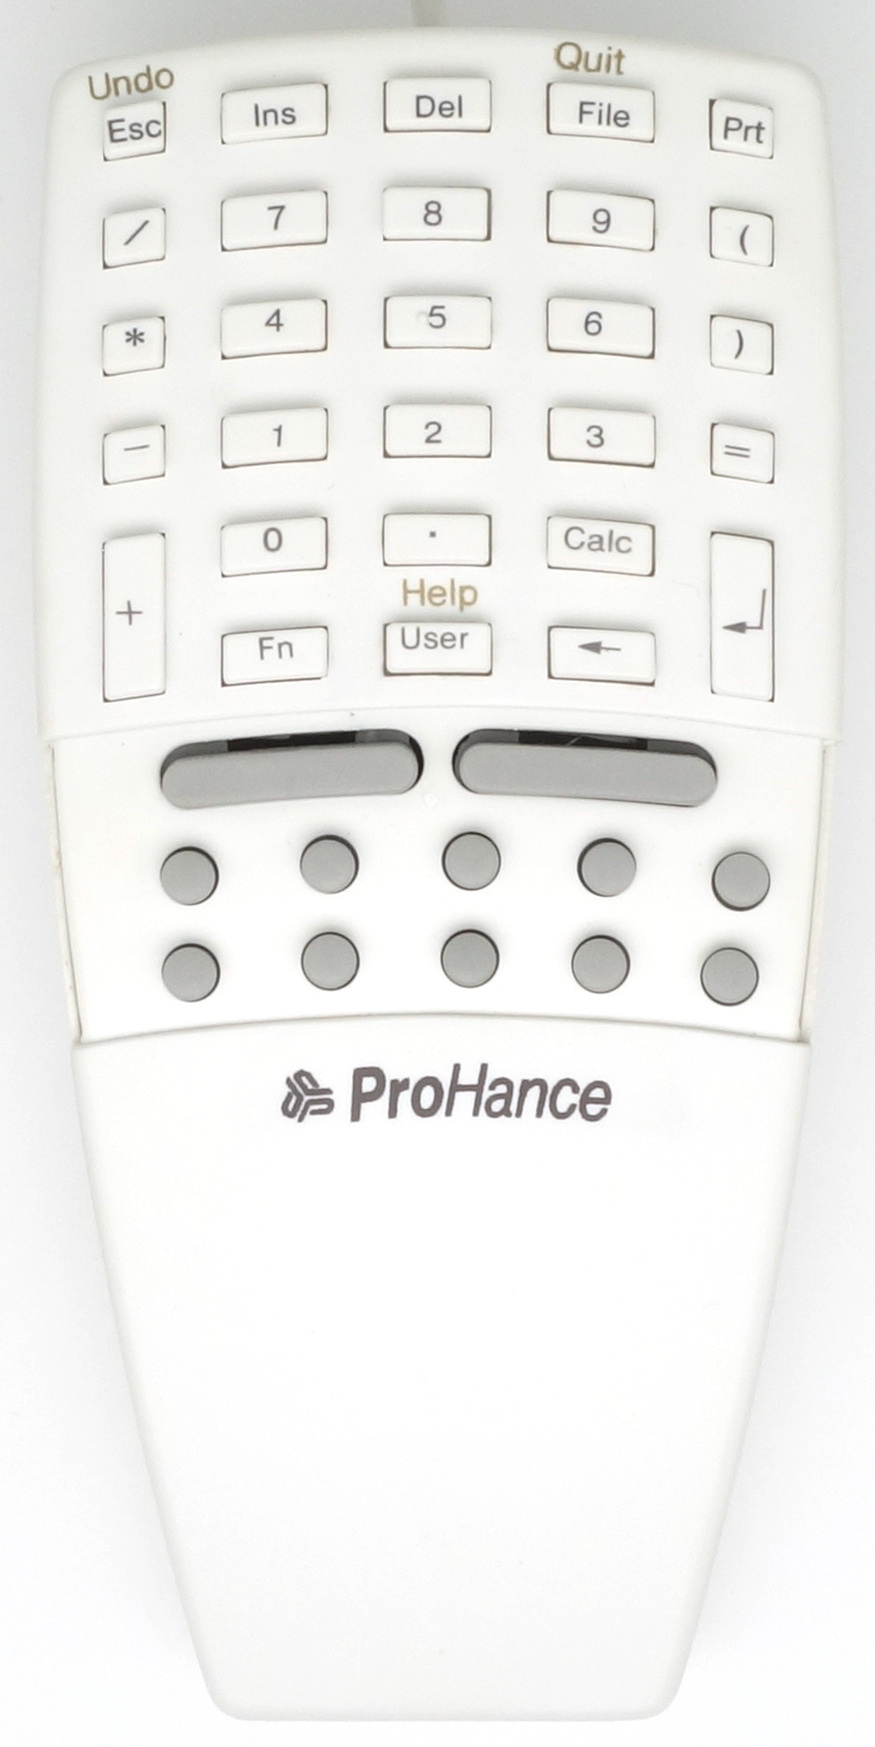
\includegraphics[scale=0.51]{1989_prohance_powermouse_100/top1_30.jpg}
    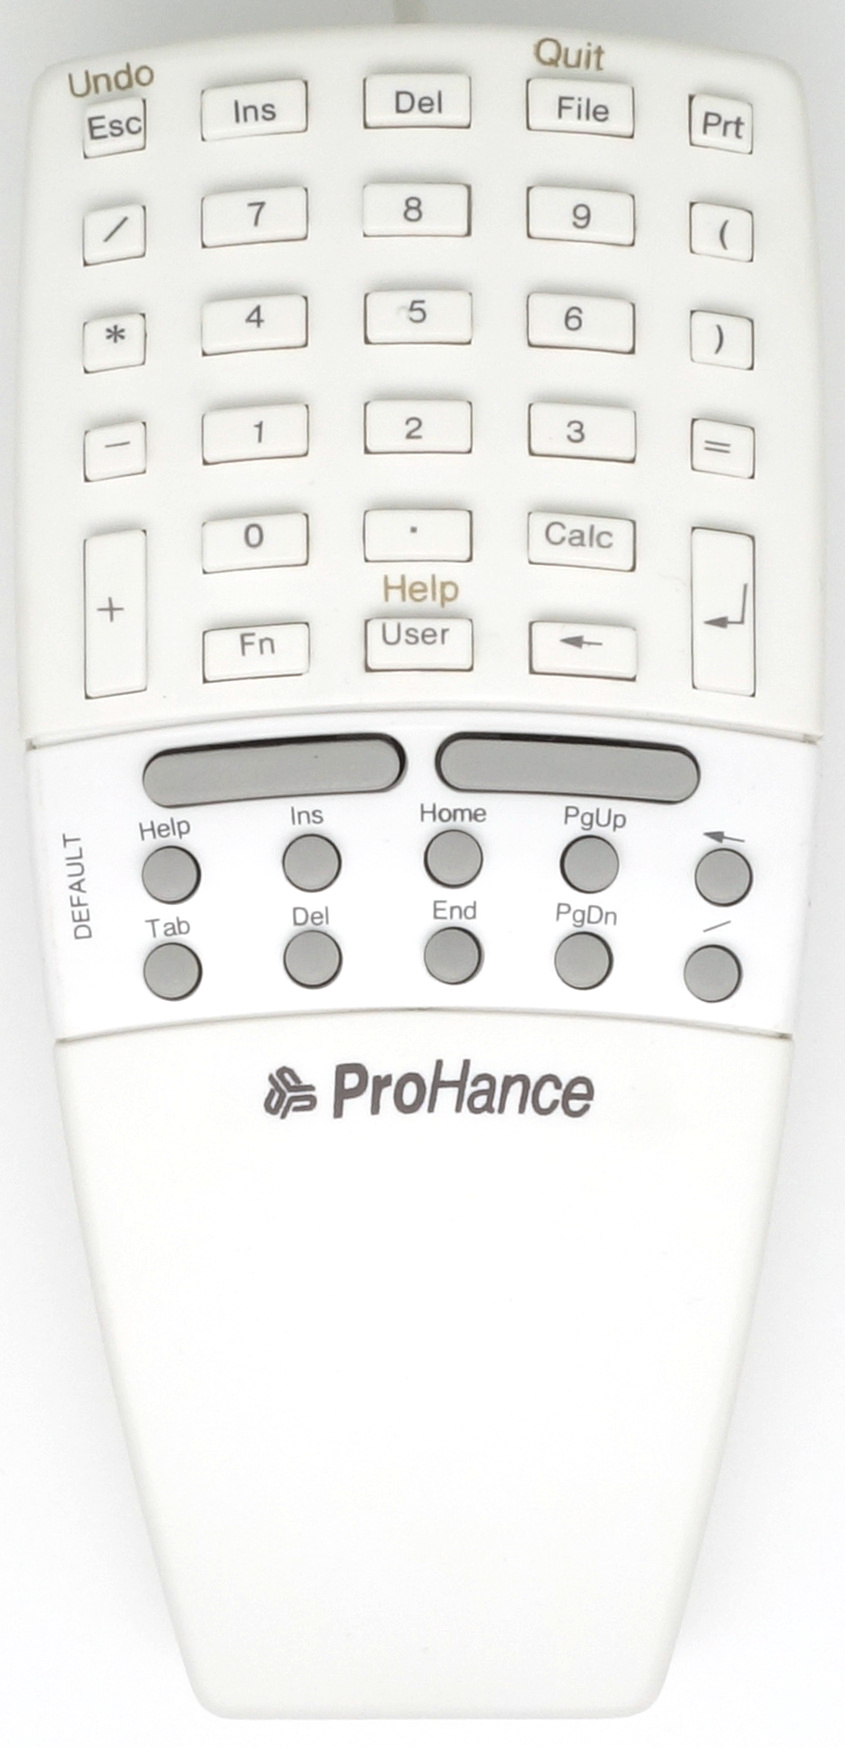
\includegraphics[scale=0.51]{1989_prohance_powermouse_100/top2_30.jpg}
    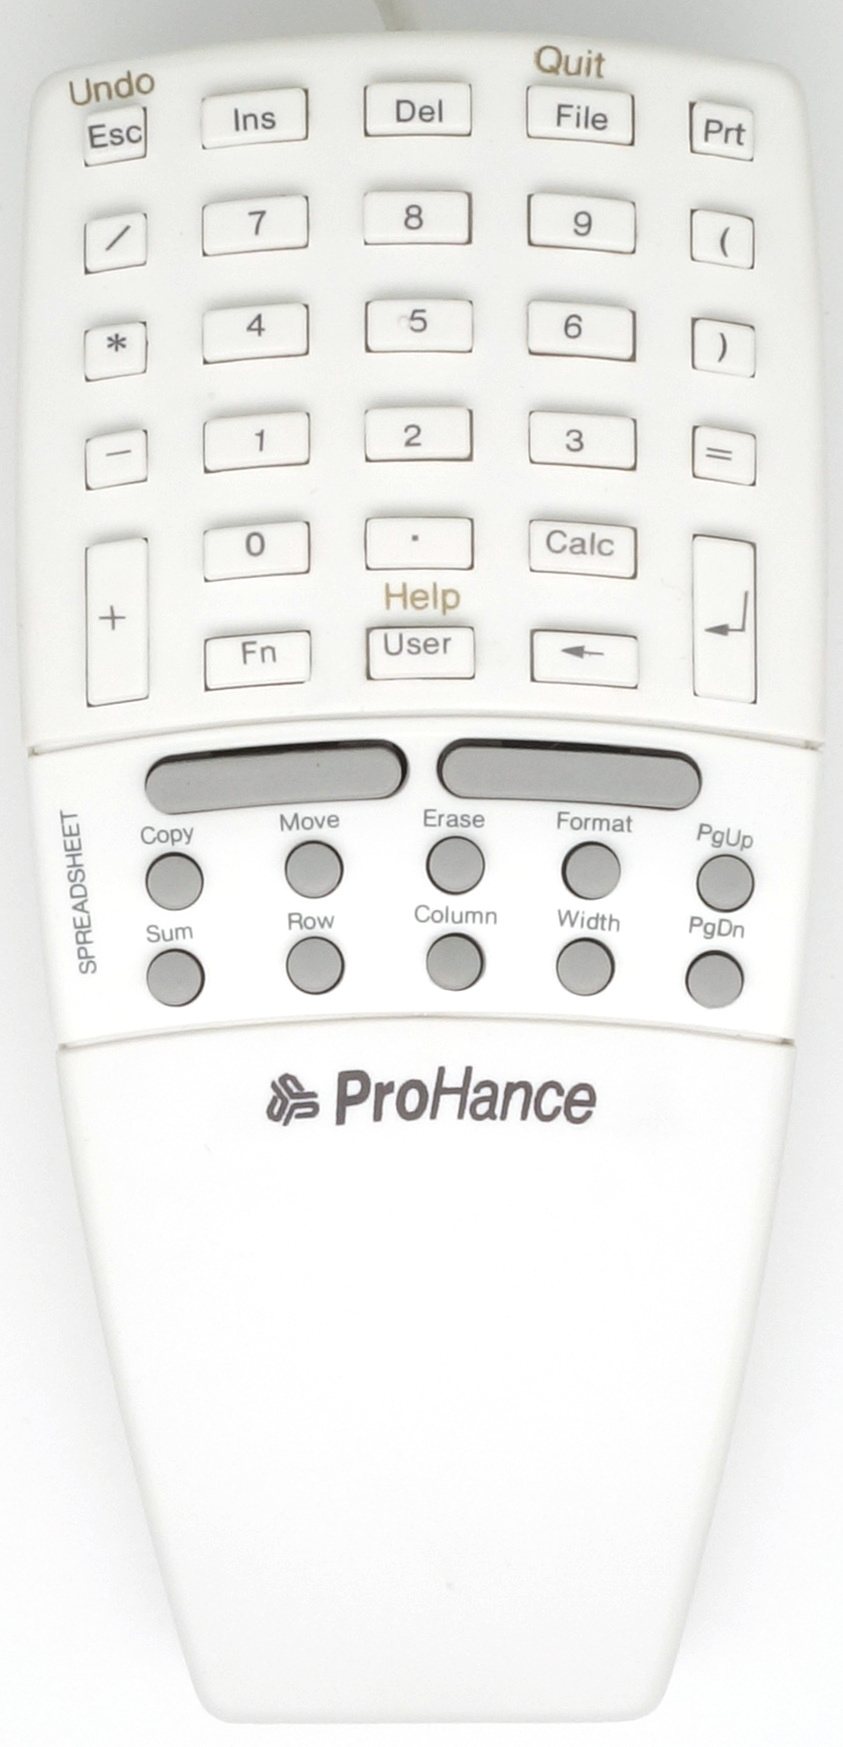
\includegraphics[scale=0.51]{1989_prohance_powermouse_100/top3_30.jpg}
    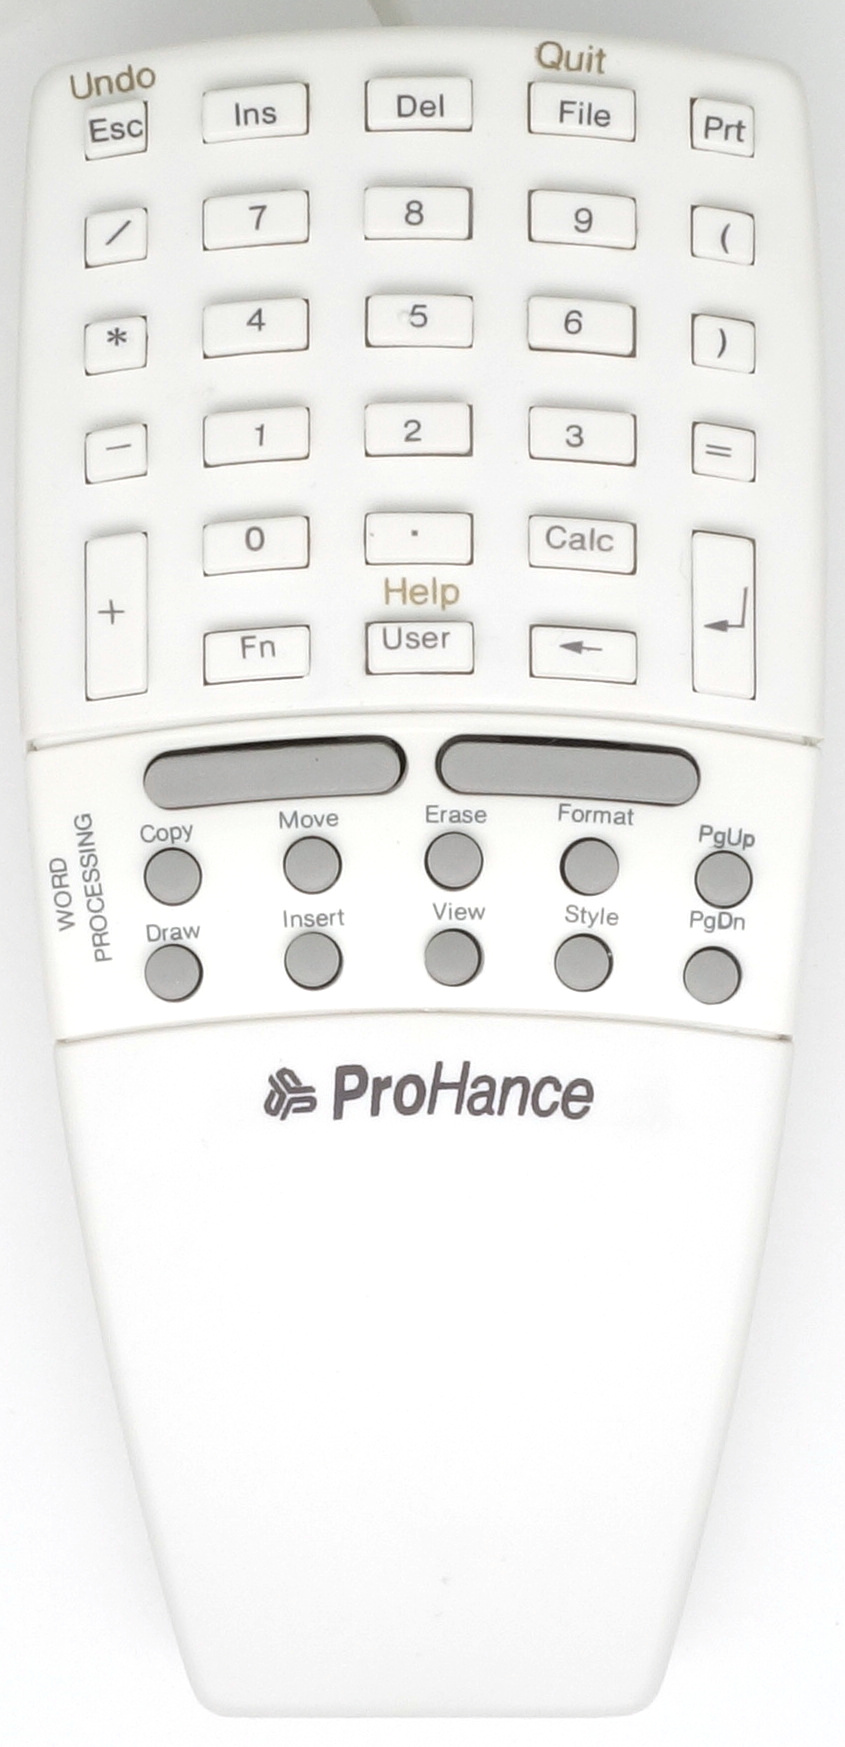
\includegraphics[scale=0.51]{1989_prohance_powermouse_100/top4_30.jpg}
    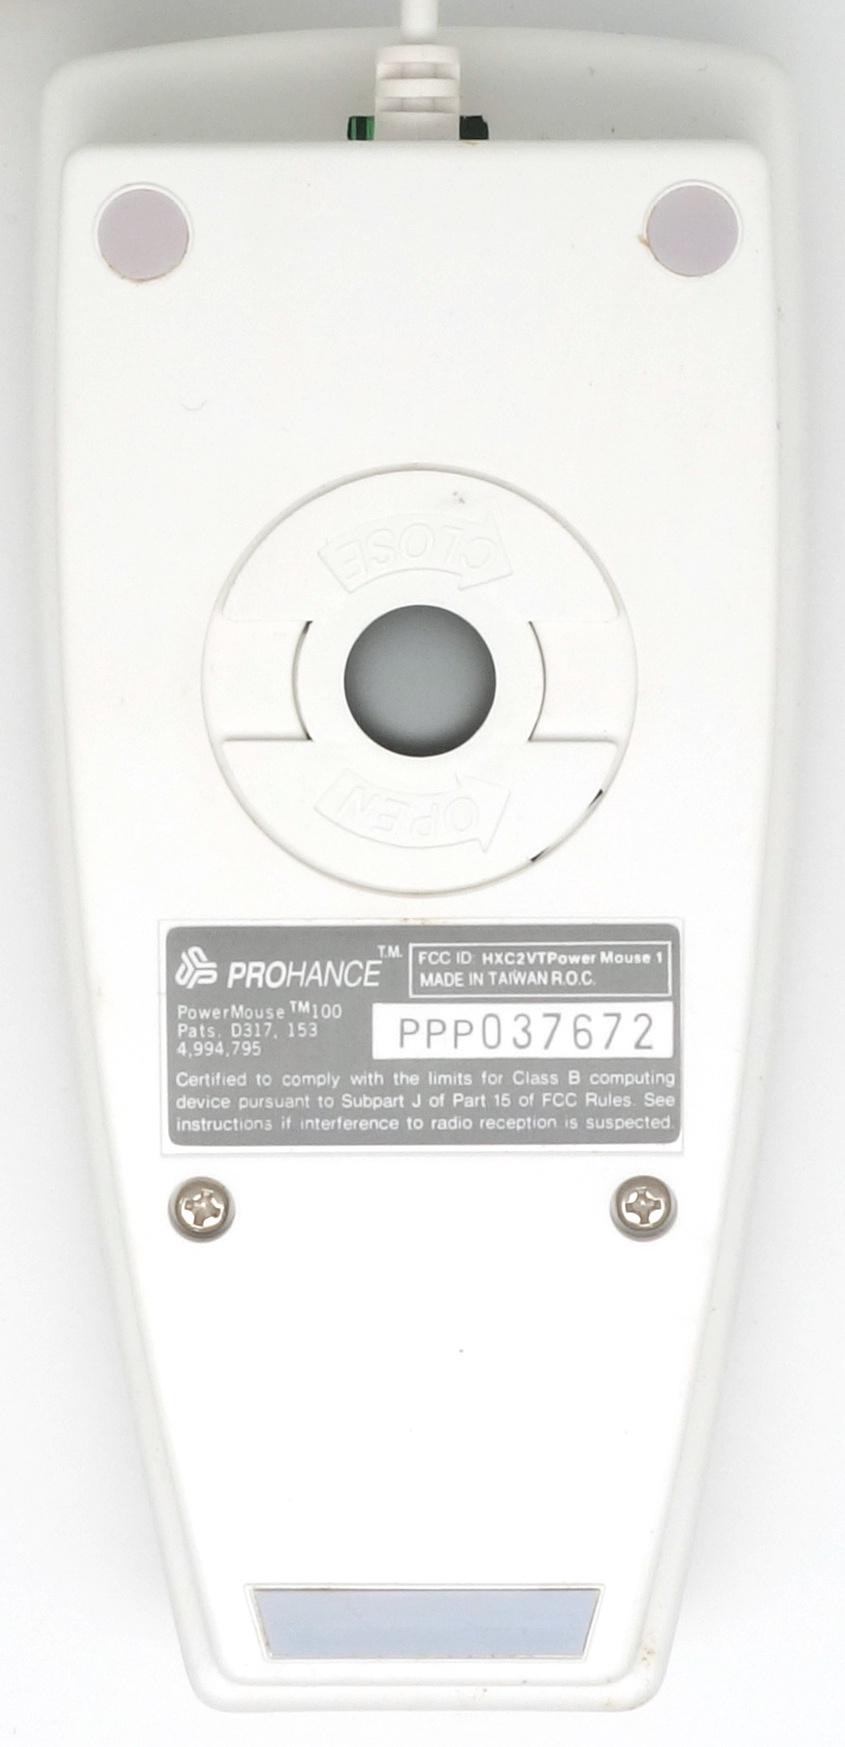
\includegraphics[scale=0.51]{1989_prohance_powermouse_100/bottom1_30.jpg}
    \caption{Prohance PowerMouse 100 later version, top and bottom views}
    \label{fig:ProhanceTopAndBottom2}
\end{figure}


Prohance mentions that 1992 version of the mouse supports ``word processing, spreadsheet, CAD, desktop publishing, database, drawing, and more''. Their support consists of the fact that when a mouse function key is pressed, the driver generates a specified sequence of keyboard and mouse events -- in fact, a button press results in a macro command. MS DOS compatible configuration software provided by Prohance allows to switch sets of these macro commands, or to create new ones \cite{manual}: 6 definable tasks per button (using Shift, Ctrl, Alt, etc.). Otherwise, this pointing device acts like any other mouse. As \cite{prohance} notes, the earlier version of the driver contained errors that caused the mouse to work inadequately in Microsoft Word (even its slight movement led to page scrolling), which were fixed in the updated version. There was also some software incompatibility with the Microsoft mouse driver, which resulted in the mouse not working with some applications. The driver also allowed the user to adjust the mouse sensitivity level via the configuration file, however dynamic regulation of mouse acceleration has not been implemented.


\begin{figure}[h]
    \centering
    
\includegraphics[scale=0.34]{1989_prohance_powermouse_100/size_30.jpg}
    \caption{Prohance PowerMouse 100 on a graduated pad with a grid step of 1~cm}
    \label{fig:ProhanceSize}
\end{figure}

The Prohance PoverMouse 100's size (figure \ref{fig:ProhanceSize}) doesn't give it the best ergonomics; however, this is not the only problem of this mouse. An important drawback is the size of the buttons: both the two main buttons and the additional Prohance keys have too small area. 

The keycaps are made of rubber, like the buttons of a pocket calculator, but they make a barely audible click when pressed (still, the key travel is rather big, so the probability of accidentally pressing a key is small).

Keycaps have no tactile or visual distinguishing features. This is especially problematic for function keys: they have round caps of the same size, so you need to carefully monitor the correct position of your finger before pressing. 
Replaceable covers placed in the functional keys section allow visual identification of keys in different operating modes. However, the labels on them are small, fingers overlap them, and an untrained user has to look closely to find the right one (the difference in the size of the fingertip and the function button is clearly visible in figure \ref{fig:ProhanceHand}).

\begin{figure}[h]
    \centering
    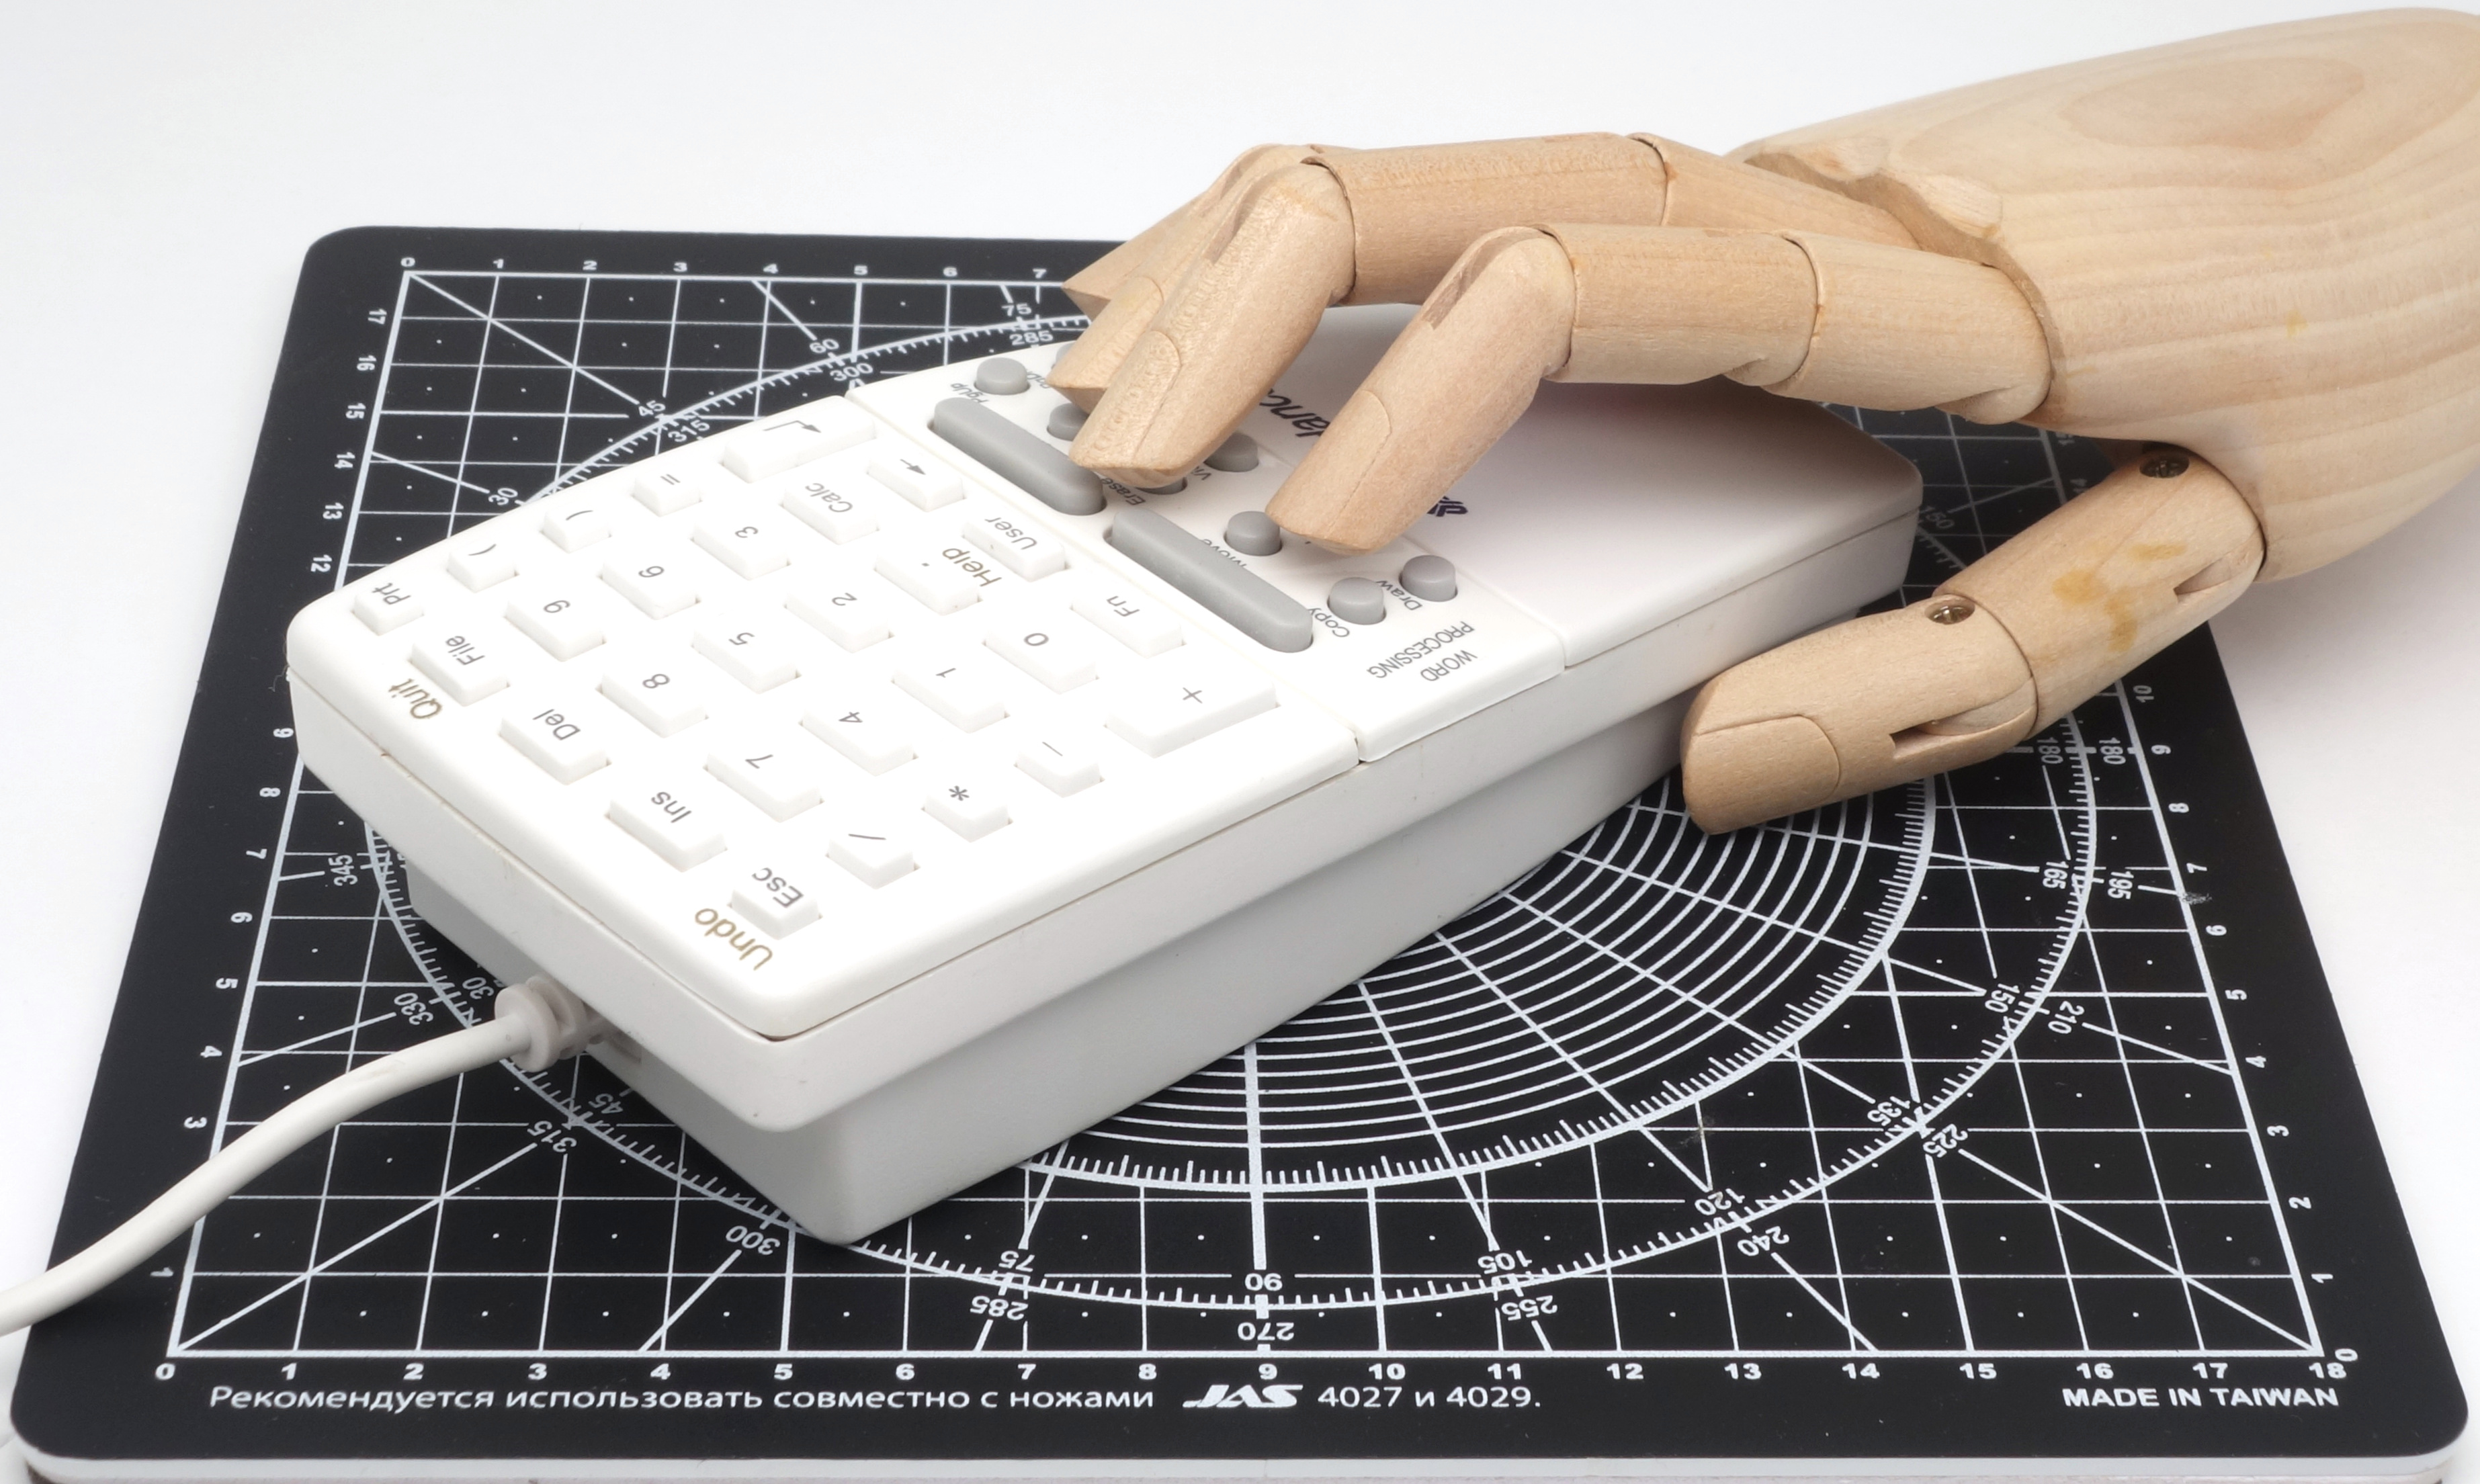
\includegraphics[scale=0.4]{1989_prohance_powermouse_100/hand2_15.jpg}
    \caption{Prohance PowerMouse 100 with a human hand model}
    \label{fig:ProhanceHand}
\end{figure}

The manufacturer touted the ergonomic advantage of allowing users no longer had to ``waste time or lose concentration going back and forth to the keyboard or to pop-down menus'' \cite{box}. However, in exchange, they had to contend with pressing extremely narrow left and right mouse buttons and squinting at the tiny labels between the keys, which did not add to the mouse's positive reviews.

\begin{figure}[h]
    \centering
    
\includegraphics[scale=0.8]{1989_prohance_powermouse_100/inside_60.jpg}
    \caption{Prohance PowerMouse 100 disassembled}
    \label{fig:ProhanceInside}
\end{figure}

Mouse internals are shown on figure \ref{fig:ProhanceInside}. It is an opto-mechanical device typical for the beginning of the 90s, and the buttons and functional keys block is made on a separate printed circuit board: it is a miniature membrane keyboard similar to installed in pocket calculators.

\begin{thebibliography}{9}
\bibitem{livingston} Livingston B. Genetically engineered mice run amok at Windows World // InfoWorld, Vol. 15, Iss. 21, May 24, 1989. - p. 34. \url{https://books.google.by/books?id=PTsEAAAAMBAJ&lpg=PA34&dq=prohance%20mouse&hl=ru&pg=PA34#v=onepage&q=prohance%20mouse&f=false}
\bibitem{pcmag} Mouse Integrates Numeric Keypad, Programmable Keys // PC Magazine, V. 8, Iss. 12, June 27, 1989. - P. 56. \url{https://archive.org/details/PC-Mag-1989-06-27/page/n57/mode/2up}
\bibitem{prohance} Gruman G. What price mice? // Infoworld, V. 12, No. 17, April 23, 1990. - P. 63-69. \url{https://books.google.by/books?id=LTsEAAAAMBAJ&lpg=PA63&ots=GzwI8rKvl3&dq=%22prohance%20powermouse%22&pg=PA63#v=onepage&q&f=false}
\bibitem{box} Prohance PowerMouse 100 [the box] \url{raw.githubusercontent.com/fiowro/mouses/main/source/OCR/prohance_powermouse_100_box.pdf}
\bibitem{manual} Prohance PowerMouse and PowerTrack User's guide \url{raw.githubusercontent.com/fiowro/mouses/main/source/OCR/prohance_powermouse_powertrack_manual.pdf}
\end{thebibliography}
\end{document}

